\documentclass[fleqn]{article}
\oddsidemargin 0.0in
\textwidth 6.0in
\thispagestyle{empty}
\usepackage{import}
\usepackage{amsmath}
\usepackage{graphicx}
\usepackage{flexisym}
\usepackage{calligra}
\usepackage{amssymb}
\usepackage{bigints} 
\usepackage[english]{babel}
\usepackage[utf8x]{inputenc}
\usepackage{float}
\usepackage[colorinlistoftodos]{todonotes}


\DeclareMathAlphabet{\mathcalligra}{T1}{calligra}{m}{n}
\DeclareFontShape{T1}{calligra}{m}{n}{<->s*[2.2]callig15}{}
\newcommand{\scriptr}{\mathcalligra{r}\,}
\newcommand{\boldscriptr}{\pmb{\mathcalligra{r}}\,}

\definecolor{hwColor}{HTML}{442020}

\begin{document}

  \begin{titlepage}

    \newcommand{\HRule}{\rule{\linewidth}{0.5mm}}

    \center

    \begin{center}
      
\includegraphics[height=11cm, width=11cm]{asu.png}
    \end{center}

    \vline

    \textsc{\LARGE Statistical/Thermal Physics}\\[1.5cm]

    \HRule \\[0.5cm]
    { \huge \bfseries Homework 13}\\[0.4cm] 
    \HRule \\[1.0cm]

    \textbf{Behnam Amiri}

    \bigbreak

    \textbf{Prof: Michael Treacy}

    \bigbreak

    \textbf{{\large \today}\\[2cm]}

    \vfill

  \end{titlepage}

  \begin{enumerate}
    \item \textbf{7.3}

      \begin{center}
        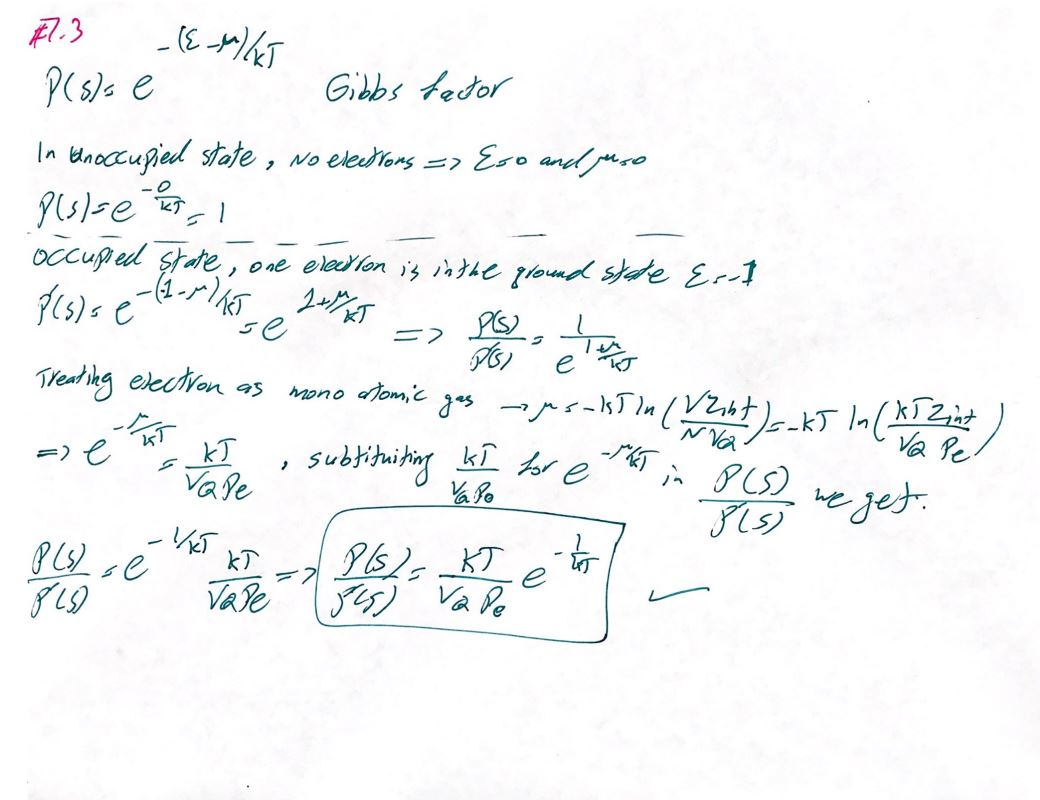
\includegraphics[height=16cm, width=17cm]{73.JPG}
      \end{center}

    \pagebreak
    
    \item \textbf{7.4}

    \begin{center}
      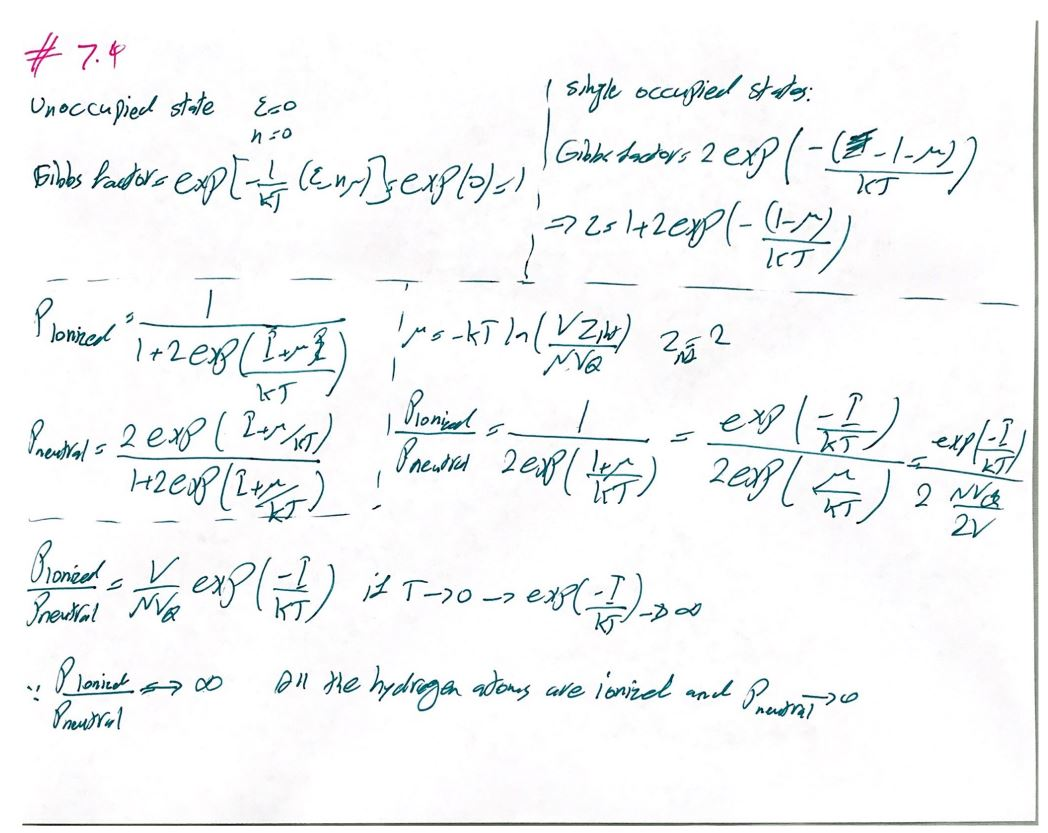
\includegraphics[height=16cm, width=17cm]{74.JPG}
    \end{center}
    
    \pagebreak

    \item \textbf{7.6}

    \begin{center}
      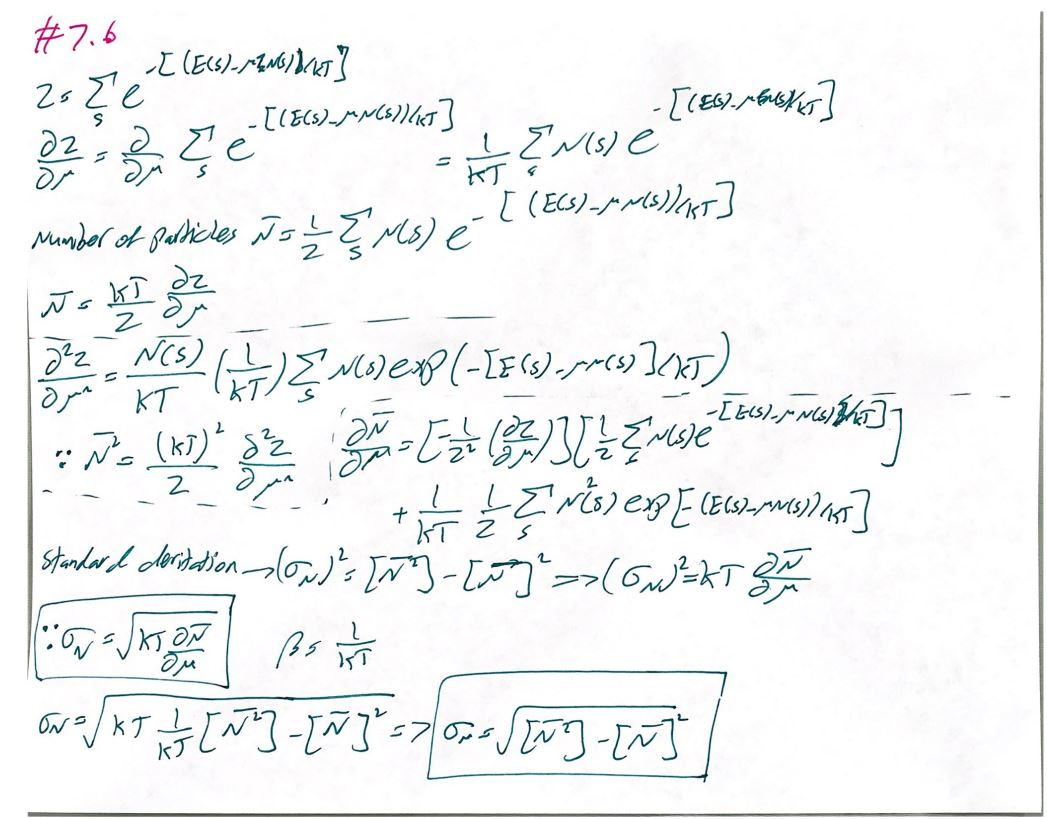
\includegraphics[height=16cm, width=17cm]{76.JPG}
    \end{center}
    
    \pagebreak

    \item \textbf{7.8}

    \begin{center}
      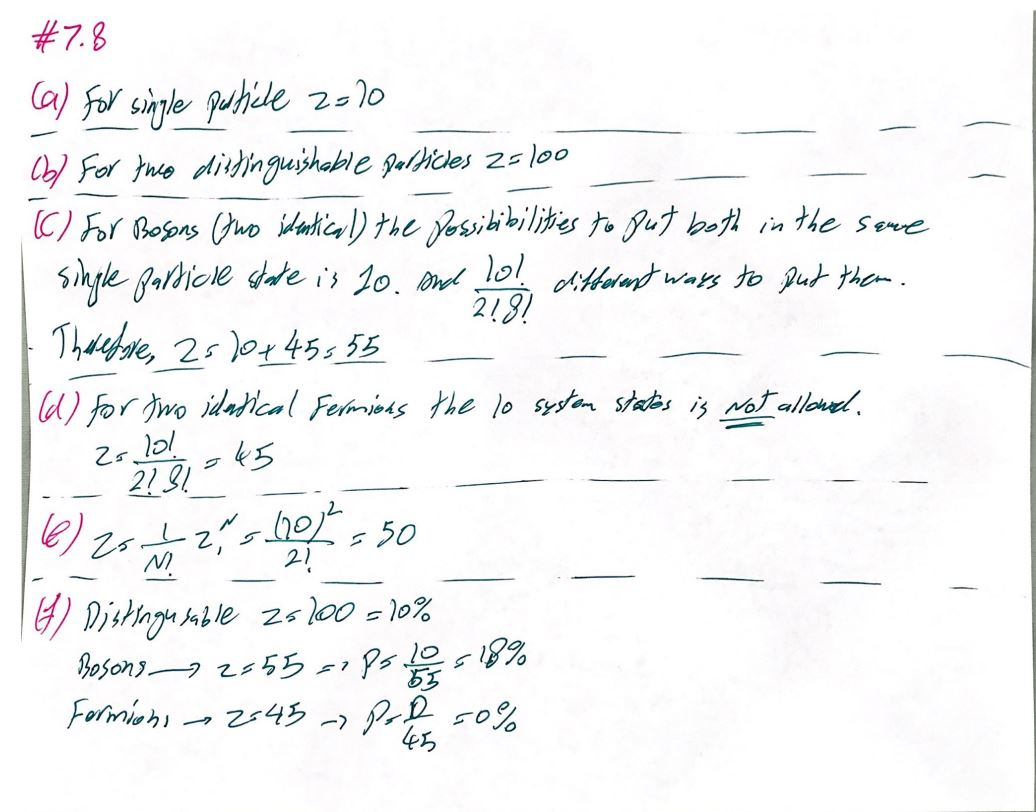
\includegraphics[height=16cm, width=17cm]{78.JPG}
    \end{center}
    
    \pagebreak

    \item \textbf{7.9}

    \begin{center}
      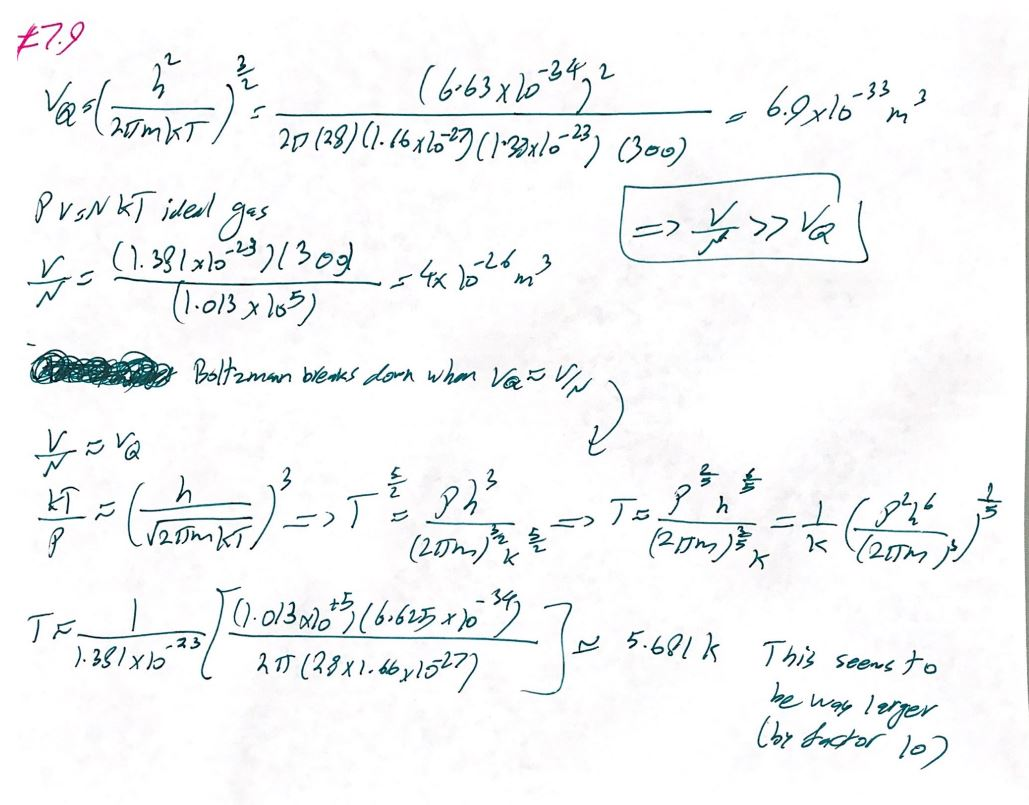
\includegraphics[height=16cm, width=17cm]{79.JPG}
    \end{center}
    
    \pagebreak

    \item \textbf{7.10}

    \begin{center}
      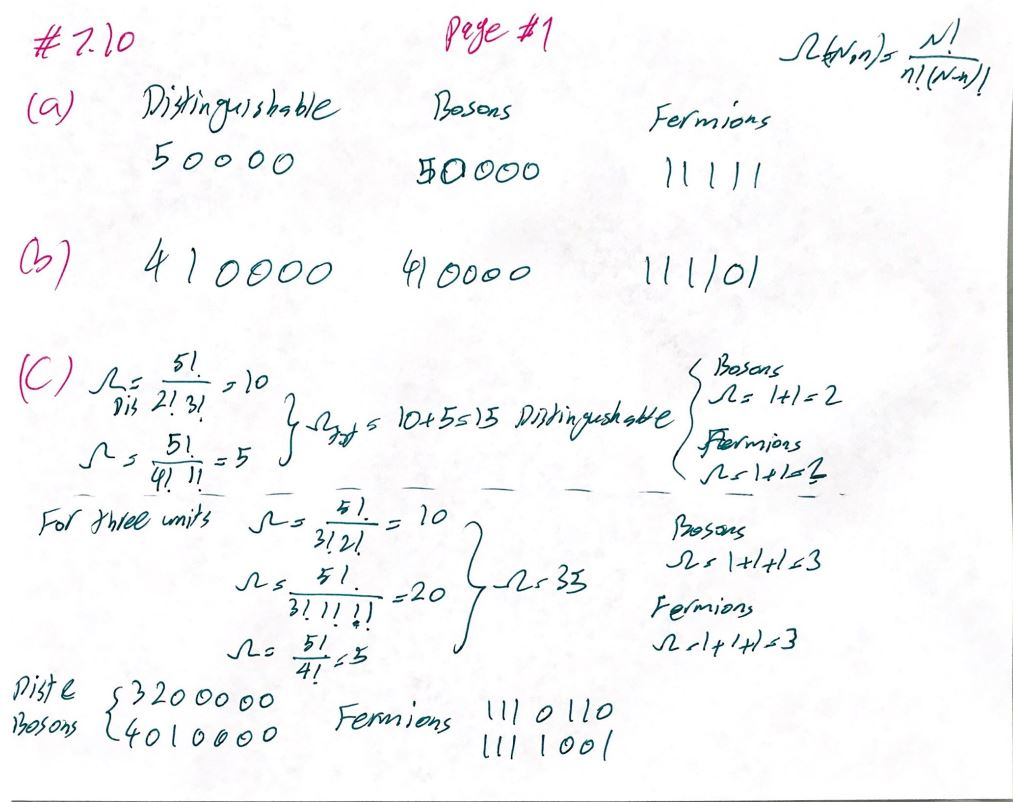
\includegraphics[height=16cm, width=17cm]{710A.JPG}
    \end{center}
    
    \pagebreak

    \begin{center}
      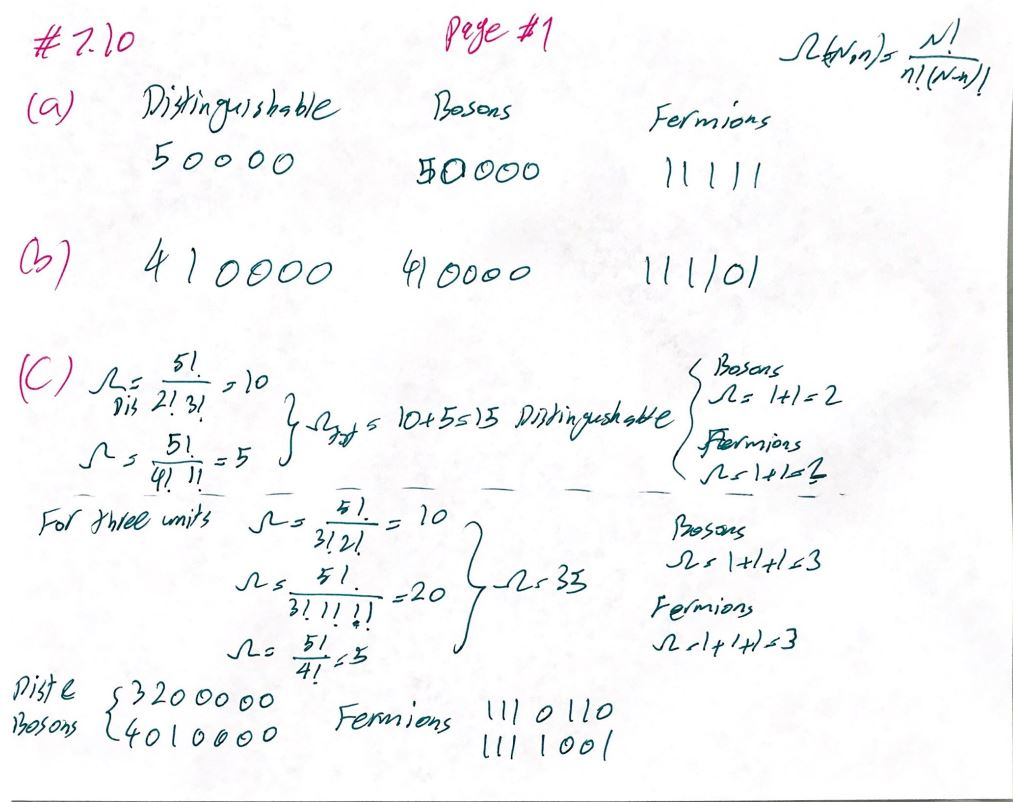
\includegraphics[height=16cm, width=17cm]{710A.JPG}
    \end{center}
    

  \end{enumerate}

\end{document}
